\documentclass{article}

\usepackage{url}
\usepackage{tikz}
\usepackage{float}
\usepackage{amsmath}
\usetikzlibrary{matrix, shapes, snakes}

\title{CS 510: Midterm\\Fall 2012}

\author{Dustin Ingram}

\date{\today}

\begin{document}

\maketitle

\begin{enumerate}

\item{} % 1

\begin{enumerate}

\item{\textbf{False} A ``pure reflex agent'' by definition does not make
decisions based on previous states of the environment, nor does it have a model
or internal representation of the environment, which are key characteristics
that a knowledge-based agent uses to choose an agent's actions.}

\item{\textbf{True}: A BFS search is guaranteed to arrive at a solution if the
branching factor is finite. Although the depth may be infinite, the search will
not fall into a cycle like a DFS search would because it does not evaluate
states consecutively.}

\item{\textbf{False}: A* used bi-directionally would provide no additional
benefit, and would create additional overhead for the search algorithm.}

\item{\textbf{True}: While it is possible to write a heuristic function which
always returns the exact minimum cost of solving the puzzle, this function
would essentially amount to solving the puzzle and thus not be a very useful 
heuristic.}

\end{enumerate}

\item{} % 2

\begin{enumerate}

\item{Via depth-first search:}

\begin{figure}[H]
\centering
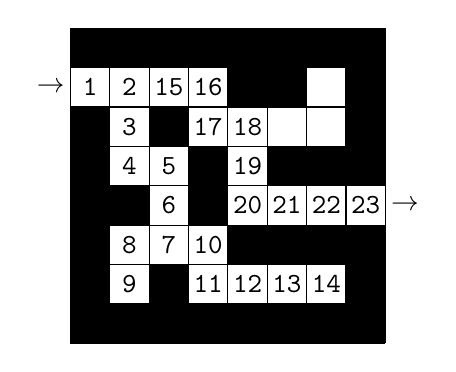
\begin{tikzpicture}
\draw[step=0.5cm,color=black] (-2,-2) grid (2,2);
        \node[fill=black,minimum width=4cm,minimum height=0.5cm] at (0,-1.75) {};
        \node[fill=black,minimum width=4cm,minimum height=0.5cm] at (0,1.75) {};
        \node[fill=black,minimum width=2cm,minimum height=0.5cm] at (1.0,-.75) {};
        \node[fill=black,minimum width=1cm,minimum height=0.5cm] at (1.0,.25) {};
        \node[fill=black,minimum width=1cm,minimum height=0.5cm] at (0.5,1.25) {};
        \node[fill=black,minimum width=0.5cm,minimum height=3cm] at (-1.75, -0.5) {};
        \node[fill=black,minimum width=0.5cm,minimum height=2cm] at (1.75, 1.0) {};
        \node[fill=black,minimum width=0.5cm,minimum height=1.0cm] at (1.75, -1.0) {};
        \node[fill=black,minimum width=0.50cm,minimum height=1.0cm] at (-.25, 0) {};
        \node[fill=black,minimum width=0.5cm,minimum height=0.5cm] at (-0.75,+0.75) {};
        \node[fill=black,minimum width=0.5cm,minimum height=0.5cm] at (-1.25,-.25) {};
        \node[fill=black,minimum width=0.5cm,minimum height=0.5cm] at (-.75,-1.25) {};
        \node at (-2.25,1.25) {$\rightarrow$};
        \node at (2.25,-.25) {$\rightarrow$};
        \node at (-1.75,1.25) {\texttt{1}};
        \node at (-1.25,1.25) {\texttt{2}};
        \node at (-.75,1.25) {\texttt{15}};
        \node at (-.25,1.25) {\texttt{16}};
        \node at (1.25,1.25) {};
        \node at (-1.25,+0.75) {\texttt{3}};
        \node at (-0.25,+0.75) {\texttt{17}};
        \node at (+0.25,+0.75) {\texttt{18}};
        \node at (+0.75,+0.75) {};
        \node at (+1.25,+0.75) {};
        \node at (-1.25,+0.25) {\texttt{4}};
        \node at (-0.75,+0.25) {\texttt{5}};
        \node at (-0.75,-0.25) {\texttt{6}};
        \node at (+0.25,+0.25) {\texttt{19}};
        \node at (+0.25,-0.25) {\texttt{20}};
        \node at (+0.75,-0.25) {\texttt{21}};
        \node at (+1.25,-0.25) {\texttt{22}};
        \node at (+1.75,-0.25) {\texttt{23}};
        \node at (-0.75,-0.75) {\texttt{7}};
        \node at (-0.25,-0.75) {\texttt{10}};
        \node at (-1.25,-0.75) {\texttt{8}};
        \node at (-1.25,-1.25) {\texttt{9}};
        \node at (-0.25,-1.25) {\texttt{11}};
        \node at (0.25,-1.25) {\texttt{12}};
        \node at (0.75,-1.25) {\texttt{13}};
        \node at (1.25,-1.25) {\texttt{14}};
\end{tikzpicture}
\end{figure}

\item{Via breadth-first search:}

\begin{figure}[H]
\centering
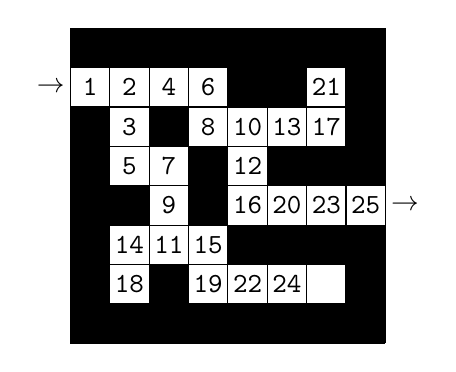
\begin{tikzpicture}
\draw[step=0.5cm,color=black] (-2,-2) grid (2,2);
        \node[fill=black,minimum width=4cm,minimum height=0.5cm] at (0,-1.75) {};
        \node[fill=black,minimum width=4cm,minimum height=0.5cm] at (0,1.75) {};
        \node[fill=black,minimum width=2cm,minimum height=0.5cm] at (1.0,-.75) {};
        \node[fill=black,minimum width=1cm,minimum height=0.5cm] at (1.0,.25) {};
        \node[fill=black,minimum width=1cm,minimum height=0.5cm] at (0.5,1.25) {};
        \node[fill=black,minimum width=0.5cm,minimum height=3cm] at (-1.75, -0.5) {};
        \node[fill=black,minimum width=0.5cm,minimum height=2cm] at (1.75, 1.0) {};
        \node[fill=black,minimum width=0.5cm,minimum height=1.0cm] at (1.75, -1.0) {};
        \node[fill=black,minimum width=0.50cm,minimum height=1.0cm] at (-.25, 0) {};
        \node[fill=black,minimum width=0.5cm,minimum height=0.5cm] at (-0.75,+0.75) {};
        \node[fill=black,minimum width=0.5cm,minimum height=0.5cm] at (-1.25,-.25) {};
        \node[fill=black,minimum width=0.5cm,minimum height=0.5cm] at (-.75,-1.25) {};
        \node at (-2.25,1.25) {$\rightarrow$};
        \node at (2.25,-.25) {$\rightarrow$};
        \node at (-1.75,1.25) {\texttt{1}};
        \node at (-1.25,1.25) {\texttt{2}};
        \node at (-.75,1.25) {\texttt{4}};
        \node at (-.25,1.25) {\texttt{6}};
        \node at (1.25,1.25) {\texttt{21}};
        \node at (-1.25,+0.75) {\texttt{3}};
        \node at (-0.25,+0.75) {\texttt{8}};
        \node at (+0.25,+0.75) {\texttt{10}};
        \node at (+0.75,+0.75) {\texttt{13}};
        \node at (+1.25,+0.75) {\texttt{17}};
        \node at (-1.25,+0.25) {\texttt{5}};
        \node at (-0.75,+0.25) {\texttt{7}};
        \node at (-0.75,-0.25) {\texttt{9}};
        \node at (+0.25,+0.25) {\texttt{12}};
        \node at (+0.25,-0.25) {\texttt{16}};
        \node at (+0.75,-0.25) {\texttt{20}};
        \node at (+1.25,-0.25) {\texttt{23}};
        \node at (+1.75,-0.25) {\texttt{25}};
        \node at (-0.75,-0.75) {\texttt{11}};
        \node at (-0.25,-0.75) {\texttt{15}};
        \node at (-1.25,-0.75) {\texttt{14}};
        \node at (-1.25,-1.25) {\texttt{18}};
        \node at (-0.25,-1.25) {\texttt{19}};
        \node at (0.25,-1.25) {\texttt{22}};
        \node at (0.75,-1.25) {\texttt{24}};
        \node at (1.25,-1.25) {};
\end{tikzpicture}
\end{figure}

\item{This heuristic is admissible -- it will never overestimate the cost to
reach the goal. The minimum possible cost to reach the goal from any position
is the sum of the number of rows between $n$ and the exit cell and the columns
between $n$ and the exit cell. Since the heuristic $h(n)$ only takes the number
of rows into account, and because the number of columns cannot be negative, in
a maze with no obstacles, the heuristic would give a cost less than or exactly
equal to the actual cost.}

\item{Via A* search:}

\begin{figure}[H]
\centering
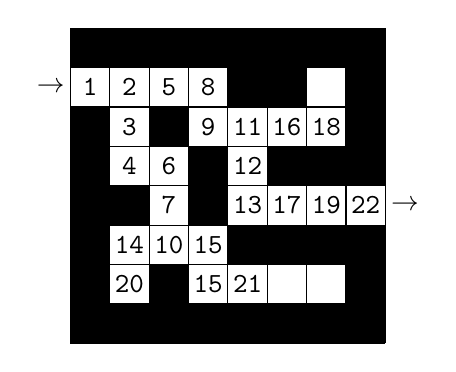
\begin{tikzpicture}
\centering
\draw[step=0.5cm,color=black] (-2,-2) grid (2,2);
        \node[fill=black,minimum width=4cm,minimum height=0.5cm] at (0,-1.75) {};
        \node[fill=black,minimum width=4cm,minimum height=0.5cm] at (0,1.75) {};
        \node[fill=black,minimum width=2cm,minimum height=0.5cm] at (1.0,-.75) {};
        \node[fill=black,minimum width=1cm,minimum height=0.5cm] at (1.0,.25) {};
        \node[fill=black,minimum width=1cm,minimum height=0.5cm] at (0.5,1.25) {};
        \node[fill=black,minimum width=0.5cm,minimum height=3cm] at (-1.75, -0.5) {};
        \node[fill=black,minimum width=0.5cm,minimum height=2cm] at (1.75, 1.0) {};
        \node[fill=black,minimum width=0.5cm,minimum height=1.0cm] at (1.75, -1.0) {};
        \node[fill=black,minimum width=0.5cm,minimum height=1.0cm] at (-.25, 0) {};
        \node[fill=black,minimum width=0.5cm,minimum height=0.5cm] at (-0.75,+0.75) {};
        \node[fill=black,minimum width=0.5cm,minimum height=0.5cm] at (-1.25,-.25) {};
        \node[fill=black,minimum width=0.5cm,minimum height=0.5cm] at (-.75,-1.25) {};
        \node at (-2.25,1.25) {$\rightarrow$};
        \node at (2.25,-.25) {$\rightarrow$};
        \node at (-1.75,1.25) {\texttt{1}};
        \node at (-1.25,1.25) {\texttt{2}};
        \node at (-.75,1.25) {\texttt{5}};
        \node at (-.25,1.25) {\texttt{8}};
        \node at (1.25,1.25) {};
        \node at (-1.25,+0.75) {\texttt{3}};
        \node at (-0.25,+0.75) {\texttt{9}};
        \node at (+0.25,+0.75) {\texttt{11}};
        \node at (+0.75,+0.75) {\texttt{16}};
        \node at (+1.25,+0.75) {\texttt{18}};
        \node at (-1.25,+0.25) {\texttt{4}};
        \node at (-0.75,+0.25) {\texttt{6}};
        \node at (-0.75,-0.25) {\texttt{7}};
        \node at (+0.25,+0.25) {\texttt{12}};
        \node at (+0.25,-0.25) {\texttt{13}};
        \node at (+0.75,-0.25) {\texttt{17}};
        \node at (+1.25,-0.25) {\texttt{19}};
        \node at (+1.75,-0.25) {\texttt{22}};
        \node at (-0.75,-0.75) {\texttt{10}};
        \node at (-0.25,-0.75) {\texttt{15}};
        \node at (-1.25,-0.75) {\texttt{14}};
        \node at (-1.25,-1.25) {\texttt{20}};
        \node at (-0.25,-1.25) {\texttt{15}};
        \node at (0.25,-1.25) {\texttt{21}};
        \node at (0.75,-1.25) {};
        \node at (1.25,-1.25) {};
\end{tikzpicture}
\end{figure}

\begin{table}[H]
\centering
\begin{tabular}{|c|c|c|c|c|}
\hline
$n$ & $g(n)$ & $h(n)$ & $g(n) + h(n)$ & fringe\\ \hline
\hline
1 & 0 & 3 & 3 & \{2\}\\\hline
2 & 1 & 3 & 4 & \{3,5\}\\\hline
3 & 2 & 2 & 4 & \{4,5\}\\\hline
4 & 3 & 1 & 4 & \{5,6\}\\\hline
5 & 2 & 3 & 5 & \{6,8\}\\\hline
6 & 4 & 1 & 5 & \{7,8\}\\\hline
7 & 5 & 0 & 5 & \{8,10\}\\\hline
8 & 3 & 3 & 6 & \{9,10\}\\\hline
9 & 4 & 2 & 6 & \{10,11\}\\\hline
10 & 6 & 1 & 7 & \{11,14,15\}\\\hline
11 & 5 & 2 & 7 & \{12,14,15,16\}\\\hline
12 & 6 & 1 & 7 & \{13,14,15,16\}\\\hline
13 & 7 & 0 & 7 & \{14,15,16,17\}\\\hline
14 & 7 & 1 & 8 & \{15,16,17,20\}\\\hline
15 & 7 & 1 & 8 & \{16,17,20,21\}\\\hline
16 & 6 & 2 & 8 & \{17,18,20,21\}\\\hline
17 & 8 & 0 & 8 & \{18,19,20,21\}\\\hline
18 & 7 & 2 & 9 & \{19,20,21,23\}\\\hline
19 & 9 & 0 & 9 & \{20,21,22,23\}\\\hline
20 & 8 & 2 & 10 & \{21,22,23\}\\\hline
21 & 8 & 2 & 10 & \{22,23\}\\\hline
22 & - & - & - & \emph{goal state}\\\hline
\end{tabular}
\caption{States of the Fringe During Every Iteration}
\end{table}


\end{enumerate}

\item{For this problem, I'm making the following assumptions: % 3

\begin{itemize}

\item that the weights and values are not known to the ``spreeer'' prior to the
start of the spree;
\item that the weights and values \emph{are} known to the ``spreeer'' during the spree;
\item that items cannot be removed from the cart once placed in it;
\item that each of the $k$ items is encountered sequentially, and only once.

\end{itemize}

This prevents the ``spreeer'' from simply determining which single item with
the best weight/value ratio which would maximize the value of a cart completely
filled with that item, either by determining this before the spree begins, by
visiting all the items in the store and returning to the most valuable item, or
by simply dumping the entire cart out when a higher-value item is found.}

\begin{enumerate}

\item{It might not make sense to encode this problem as a constraint
optimization problem because there is only a single dimension of constraint:
the total weight of the items in the cart. If another dimension, such as the
volume of the items in the cart had to be considered as well, representing this
problem as a constraint optimization problem might make sense.}

\item{Using Backtracking Search seems to be at odds with my assumptions for the
problem, as it would imply that items could be removed from the cart if it
produced a combination of items that were less favorable than a newly
encountered combination, or that items could be visited more than once.
Relaxing these assumptions, Backtracking Search would still use the fact that
there must exist an ordering of items with regards to their weight/value ratio.
An ideal heuristic would be to maximize:

\begin{equation*}
h(n) = \sum_{i=1}^n \frac{w_{i}}{v_{i}}
\end{equation*}

where $v_{i}$ is the value of a given item and $w_{i}$ is the weight, as long
as it does not exceed the total available weight of the cart. This would result
in the cart being filled with as many of the highest cost/weight item as
possible, with any remaining available space filled with the next high-value
item with a weight smaller than the available space, until the cart is full or
there are no items left which would fit.}

\item{It might be wise to solve this problem using a messy genetic algorithm:
if one were to encode each unique item as a gene value in the chromosome, the
chromosome would have varying lengths, since the cart can contain any number of
items.}

\end{enumerate}

\item{This problem would not be a good candidate for simulated annealing
search, because there is not enough variability in the ``temperature'' (i.e.,
the evaluation function $h$) to truly anneal a nearly random solution.} % 4

\item{} % 5

\begin{enumerate}

\item{There is one pure-strategy Nash equilibrium in this non-zero-sum game:
when \textsc{Player 1} chooses `A' and \textsc{Player 2} chooses `D', each
getting zero profit.}

\item{This Nash equilibrium strategy is not Pareto optimal, as there exists
other strategies which would provide both players with higher profits, namely
\{(B,E),(C,E),(B,F),(C,F)\}.}

\end{enumerate}

\item {As follows (evaluated nodes are circled in dashed gray): % 6

\begin{figure}[H]
\centering
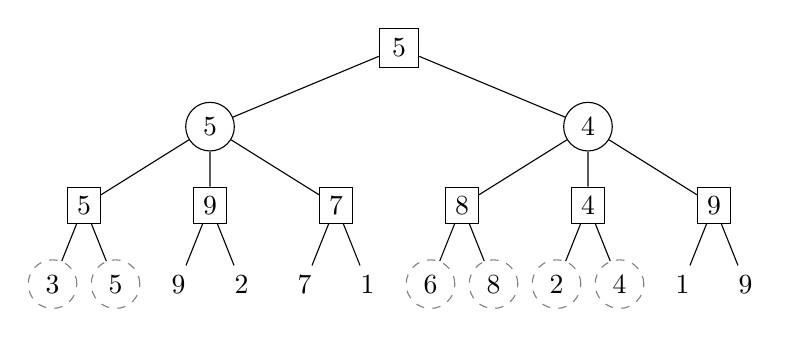
\begin{tikzpicture}[
  level 1/.style={sibling distance=48mm, level distance=10mm},
  level 2/.style={sibling distance=16mm, level distance=10mm},
  level 3/.style={sibling distance=8mm, level distance=10mm},
]
\node [rectangle,draw, minimum height=.5cm, minimum width=.5cm] (z){5}
  child {node [circle,draw] (a) {5}
    child {node [rectangle,draw] (b) {5}
      child {node [circle, dashed, draw=gray] (3) {3}}
      child {node [circle, dashed, draw=gray] (5) {5}}
    }
    child {node [rectangle,draw] (c) {9}
      child {node (9) {9}}
      child {node (2) {2}}
    }
    child {node [rectangle,draw] (d) {7}
      child {node (7) {7}}
      child {node (1) {1}}
    }
  }
  child {node [circle,draw] (j) {4}
    child {node [rectangle,draw] (k) {8}
      child {node [circle, dashed, draw=gray] (6) {6}}
      child {node [circle, dashed, draw=gray] (8) {8}}
    }
    child {node [rectangle,draw] (l) {4}
      child {node [circle, dashed, draw=gray] (2) {2}}
      child {node [circle, dashed, draw=gray] (4) {4}}
    }
    child {node [rectangle,draw] (m) {9}
      child {node (1) {1}}
      child {node (9) {9}}
    }
};
\end{tikzpicture}
\end{figure}

}

\item % 7

\begin{enumerate}

\item{Pumpkin $\pi$.}

\item{It is a quine, i.e., it outputs itself verbatim. It does this by creating
an anonymous expression which accepts a single parameter, which returns a
two-element list containing the result of the argument, and the argument fully
quoted. It then calls said anonymous function, with the fully quoted anonymous
expression as the argument.}

\item{Because \texttt{oct(31) == dec(25)}.}

\end{enumerate}

\end{enumerate}

\end{document}
